\chapter[狭义相对论]{\itr{Special relativity}{狭义相对论}}
\begin{solution}[{\large\color{plainred}Fizeau effect}\\In this problem we show that the relativistic velocity addition law can be used to
	explain the Fizeau experiment without invoking the existence of \itr{ether}{以太}. The speed of light in stationary water is less than its speed $c$ in \itr{vacuum}{真空}.
	Traditionally it is written as $\frac{c}{n}$, where $n\approx \frac{4}{3}$ is the \itr{index of refraction}{折射率} of water. The water flowed in the \itr{pipe}{管道} with
	velocity $v$. In the lower arm $T_2$ of the \itr{interferometer}{干涉仪} (as shown in the figure), one would expect that, from the nonrelativistic addition law, the
	speed of light in the moving water would be its speed in stationary
	water increased by the speed of the water in the pipe $w=\frac{c}{n}+v$. Show
	that the relativistic velocity addition law leads to, up to higher-order
	corrections:
	\begin{equation*}
		w=\frac cn+v\left(1-\frac1{n^2}\right)
	\end{equation*}
	The result was observed by Fizeau in 1851, but for long time viewed as
	a confirmation of a rather \itr{elaborate}{复杂的} \itr{contemporary}{同时代的} ether-theoretical
	calculation based on the idea that the water was partially successful in
	dragging ether along with it. Einstein later said that it was of
	fundamental importance in his thinking.]
      \begin{center}
      	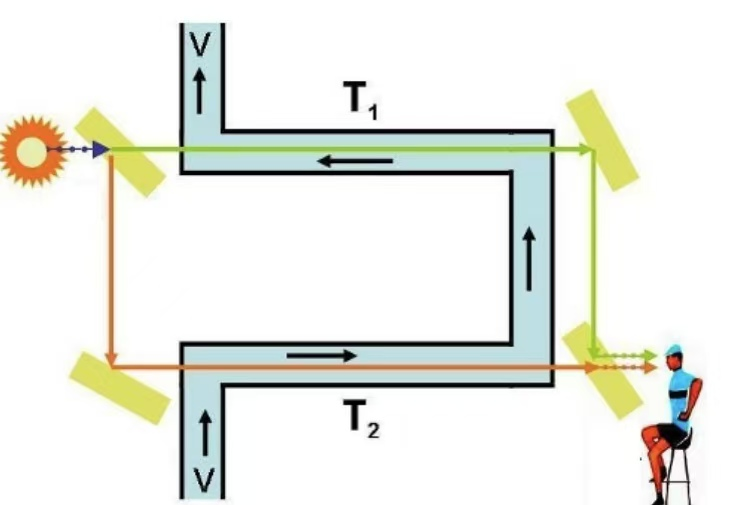
\includegraphics[width=5.5cm, height=4cm]{chapter_6_7}
      \end{center}
      此类题目主要是要选取恰当的参考系,并列出对应参数。
      
      以地面为$S$系,水流为$S^{\prime}$系,并设光前进方向为$x$轴正方向。
      
      在$S$系中,静止的水中光速为$\dfrac{c}{n}$,下方水的速度即$S^{\prime}$系相对$S$系的速度为$v$
      
      那么在$S^{\prime}$系中,由速度变换
      
      \[w=\dfrac{\dfrac{c}{n}+v}{1+\dfrac{cv}{nc^{2}}}=\dfrac{\dfrac{c}{n}+v}{1+\dfrac{v}{nc}}\]
      
      注意到$v\ll c$,故$\dfrac{v}{nc}$为小量,利用泰勒展开至一阶:
      \begin{equation*}
      	\dfrac{1}{1+\dfrac{v}{nc}} = 1 - \dfrac{v}{nc} + o\left(v^{2}\right) 
      \end{equation*}
      代入表达式中,并忽略$v^{2}$相关的高阶小量,即有:
      \[w\approx(\frac{c}{n}+v)(1-\frac{v}{nc})=\frac{c}{n}+v(1-\frac{1}{n^{2}})\]
\end{solution}
\begin{solution}[{\large\itr{Terrel Rotation}{特雷尔旋转}}\\  A square with proper-length-$L$ sides flies past you at a speed $v$, in a direction parallel to two of its sides. You stand in the plane of the square. When you see the square at its nearest point to you, show that it looks to you like it is rotated, instead of contracted. (Assume that $L$ is small compared with the distance between you and the square.)]
    \itr{Terrel Rotation}{特雷尔旋转} 是相对论效应之一,即当物体以接近光速运动时,观察者会看到物体在视觉上旋转。
    
    \ctikzfig{chapter6_solution_6_2_2}
    首先,正如图中标明的,由于尺缩效应,与运动同向的边$AB,CD$在$O$系中长度缩短为$sL$。
    
    之后,注意到我们处理的是视觉效应,那么我们就要考虑光信号到达人眼中才能成像的问题。举边$AD$为例,边上的每一个点发出的光到达人眼的时间都是不同的。在这里,我们考虑$A,D$两点。
    
    连接$AO,DO$,由于题目条件中说,人与正方形的距离远远大于$L$,可以认为$D,A,O$\\[1ex]
    近似成一条直线。因此,$A$发出的光比$D$发出的光提前$\dfrac{L}{c}$的时间到达人眼。\\[1ex]
    换而言之,人眼中接受的光信号,其实是某个时刻的$A$发出的信号,以及该时刻前\\[1ex]
    $\dfrac{L}{c}$的时刻时$D$发出的信号。人眼同时处理这两个信号,产生了“观察到$DA$边”的\\[1ex]
    效果。
    
    \ctikzfig{chapter6_solution_6_2_3}
    
    这张图中的$D_v-A_v-B_v$显示了人眼中观察到的现象。$A_vB_v$的长度即由于尺缩效\\[1ex]
    应得到的$sL$,而$A_vD_v$的长度则等于光信号时间差$\dfrac{L}{c}$乘以正方形运动的速度$v$,也\\[1ex]
    即$\beta L$。
    
    这里我们发现,恰有$(\beta L)^2 + (sL)^2 = L^2$。因此,人眼所看见的,就好像是图中旋转后的正方形$ABCD$在运动方向的投影。且对于旋转的角度$\theta$,有
    \[\sin\theta=\dfrac{\beta L}{L}=\beta\]
\end{solution}
\begin{solution}[{\large\color{plainred}Lots of transformations}\\A train with proper length $L$ moves at speed $\dfrac{c}{2}$ with respect to the ground. A ball is thrown from the back to the front, at speed $\dfrac{c}{3}$ with respect to the train. How much time does this take, and what distance does the ball cover, in:
	\\(a) The train frame?
	\\(b)The ground frame? Solve this by:
	\\\hspace*{2em}i. Using a velocity-addition argument.
	\\\hspace*{2em}ii. Using the Lorentz transformations to go from the train
	frame to the ground frame.
	\\(c)The ball frame?
	\\(d) Verify that the \itr{invariant interval}{不变(时空)间隔} is indeed the same in all three
	frames.]
        \ctikzfig{chapter6_solution_6_3}
        (a)火车相对自身是静止的,故火车系下其长度就是原长,而火车系下球的速度已知,故有
        \begin{equation*}
        	\begin{aligned}
        		&\Delta x_{1}=L\\
        		&\Delta t_{1}=\frac{L}{c/3}=\frac{3L}{c} \\
        	\end{aligned}
        \end{equation*}
        (b)选取地面为$S$系,火车为$S^{\prime}$系,火车前进方向为$x$正方向。$S^{\prime}$系相对$S$系的速度$u$为
        \[u=\dfrac{c}{2}\]
        (i)$S^{\prime}$系中球的速度为$v^{\prime}=\dfrac{c}{3}$,由速度变换公式有$S$系中,球的速度
        \[v=\dfrac{v^{\prime}+u}{1+\dfrac{{v}^{\prime}u}{c^2}}=\frac{5c}{7}\]
        列车在地面看来会发生尺缩效应,且尺缩因子$s = \sqrt{1-\left(\dfrac{u}{c}\right)^{2}} = \dfrac{\sqrt{3}}{2}$,得地面系中列车长度
        \[ d=sL = \dfrac{\sqrt{3}}{2}L\]
        在$S$系中是一个追及问题,所需时间:
        \[\Delta t_2=\frac{d}{v-u}=\frac{7\sqrt{3}L}{3c}\]
        所走距离
        \[\Delta x_2=vt_{2}=\frac{5\sqrt{3}L}{3}\]
        (ii)利用洛伦兹变换的变化量形式:
        \begin{equation*}
        	\begin{aligned}
        		&\Delta t_2 = \gamma(\Delta t_1 + \frac{u} {c^{2}}\Delta x_1)\\
        		&\Delta x_2 = \gamma(\Delta x_1 + u\Delta t_1)
        	\end{aligned}
        \end{equation*}
        可求得
        \begin{equation*}
        	\begin{aligned}
        		&\Delta t_2=\frac{7\sqrt{3}L}{3c}\\[1ex]
        		&\Delta x_2=\frac{5\sqrt{3}L}{3}\\
        	\end{aligned}
        \end{equation*}
        
        (c)在设球参考系为$S^{\prime \prime}$系,显然$S^{\prime \prime}$系下球是静止的:
        \begin{equation*}
        	\Delta x_3=0
        \end{equation*}   
        $S^{\prime \prime}$系相对$S^{\prime}$系速度$u^{\prime} = \dfrac{c}{3}$,
        有$\gamma^{\prime} = \dfrac{1}{\sqrt{1-\left(\dfrac{u^{\prime}}{c}\right)^{2}}} = \dfrac{3\sqrt{2}}{4}$,利用洛伦兹变换得
        \begin{equation*}
        	\Delta t_{3}= \gamma^{\prime}(\Delta t_1 - \frac{u^{\prime}\Delta x_1} {c^{2}})
        	=\frac{2\sqrt{2}L}{c}
        \end{equation*}
        
        (d)题意其实就是要证明时空间隔$(c\Delta t)^2-(\Delta x)^2$的不变性,将之前所求代入验证即可:
        \begin{equation*}
        	\begin{aligned}
        		(c\Delta t_{1})^{2}-(\Delta x_{1})^{2}&=8L^{2} \\
        		(c\Delta t_{2})^{2}-(\Delta x_{2})^{2}&=8L^{2}\\
        		(c\Delta t_{3})^{2}-(\Delta x_{3})^{2}&=8L^{2} \\
        	\end{aligned}
        \end{equation*}
        可见事件的时空间隔确实不变。
        
        注:如果老师上课时定义的时空间隔与此处不同,注意符号问题或者在回答时说明好。
\end{solution}
\newpage
\begin{solution}[{\large\color{plainred}Train And \itr{Tunnel}{隧道} \itr{Paradox}{悖论}}\\
	Consider a train running at a constant speed $V$ on the straight track in the $x$ direction, and passing through a tunnel (see the figure). The proper length of the train is $L$, and the proper length of the tunnel is $D$. Here we assume $L>D$. Define $(x,ct)$ as the time and the space coordinates of the track frame, and $(x',ct')$ as those of the train frame. Here, $x$ and $x' $\textbf{ are in the same direction}.	
	\\
	(a) Suppose that an observer standing on the ground sees that the train is shorter than the tunnel, so that the whole train can be inside the tunnel. Determine the smallest possible speed of the train.
	\\
	(b) Suppose that the rear end of the tunnel (see the figure) is at $x=0$, and set the time $t=t'=0$ when the rear end of the train reaches the rear end of the tunnel. Draw the Minkowski diagram \textbf{ taking $x$ coordinate for the horizontal axis and $ct$ coordinate for the vertical axis.} In addition, \itr{specify}{指明} $L$ and $D$ in the diagram.
	\\
	(c) When the rear end of the train enters the rear end of the tunnel, the rear-end and front-end sliding doors of the tunnel (see the figure) are closed at the same time in the track frame. These two events are denoted by $R_{close}$ and $F_{close}$, respectevely. Then, when the front-end of the train reaches the front end of the tunnel, both the rear-end and front-end sliding doors are opened at the same time in the track frame. These events are denoted by $R_{open}$ and $F_{open}$, respectively.
	\\
	Show the events $R_{close},F_{close},R_{open}$, and $F_{open}$ in the Minkowski diagram in (b),
	and put the four events in the order of being seen by an observer in the train.
	]
	\begin{singlefigure}{chapter_6_20}[1]    
	\end{singlefigure}
    (a)
    \\根据尺缩效应,在轨道参考系中,火车的长度为
    \[\sqrt{1-\dfrac{v^2}{c^2}}L\]
    故如需火车能够完全在隧道中,则有
    \[\sqrt{1-\dfrac{v^2}{c^2}}L\le D\]
    可解得
    \[v\ge \sqrt{1-\dfrac{D^2}{L^2}}c\]
    (b)\\
    作图如下:
    \begin{center}
    	\resizebox{16.2em}{12em}{\tikzfig{chapter6_solution_6_4_1}}
    \end{center}
    
    依据题意,隧道尾和火车尾在$0$时刻都处于$O$点。由于隧道在轨道系中静止,隧道在轨道系中的长度即为其原长$D$。因此,在$x$轴上取长度$D$,对应的$P$点即是$0$时刻时隧道头的位置。
    
    接下来,设$OQ$是$x'$轴上的,可以表示$L$的线段。
    
    首先,需要过$P$做校准曲线,与$x'$轴相交于$Q_1$点。由于题目条件$L>D$,因此$Q$在$Q_1$右侧。
    
    另外,还需要过$P$作$ct'$轴的平行线,交$x'$轴于$Q_2$点。这是因为列车在轨道系(也就是$x-ct$系)中的长度应当小于$D$,且列车头的世界线斜率与$ct'$轴斜率相同。于是,过$Q$的$ct'$轴的平行线与$x$轴的交点应在$P$的左侧,等价于$Q$在$Q_2$的左侧。
    
    综上,$Q$在$Q_1,Q_2$之间。
    
    (c)\\
    作图如下:
    \begin{center}
    	\resizebox{24em}{10em}{\tikzfig{chapter6_solution_6_4_2}}
    \end{center}
    
    由题意易知原点即代表$R_{close}$。
    
    过(b)中确定的$Q$作$ct'$的平行线,则该线即是列车头的世界线。那么,它与$x$轴的交点即代表$F_{close}$。
    
    过(b)中确定的$P$作$ct$的平行线$l$,则该线即是隧道头的世界线。那么,它与列车头世界线的交点即代表列车头到达隧道头,也即$F_{open}$
    
    题目中已说明,在轨道系中,$F_{open}$和$R_{open}$同时发生,则过$F_{open}$作$x$轴的平行线,它与$ct'$轴的交点即是$R_{open}$。
    
    由于题目要求比较在列车系中各时间的发生先后,我们取四个事件在$ct'$轴上的分量。由图即得时序为
    \[F_{close}\rightarrow F_{open}\rightarrow R_{close}\rightarrow R_{open}\]
\end{solution}
\newpage
\begin{solution}[{\large\color{plainred}Conservation of momentum in SR}\\
		In class, we showed that the classical definition of the linear
		momentum cannot be right in the relativistic case. We illustrated by the
		example of the collision of two particles with equal mass $m$. In the rest
		frame (for the center of mass) $K$, the two particles have velocities with
		the same amplitude $v$ but opposite directions along $x$ axis before the
		collision, as illustrated in Fig.(a). After the collision, they move away along $y$ axis with the same speed $v$, as illustrated in Fig.(b). \\Now, in a frame $K'$ that moves with speed $v$ along the positive $x$ direction with respect to the rest frame $K$, as illustrated in Fig.(c), one particle is at rest before the
		collision. 
		\\(i) What is the velocity of the other particle before the
		collision? 
		\\(ii) After the collision, as illustrated in Fig.(d), what are the velocities of
		the two particles? Specify the components of the velocities along $x$ and
		$y$ axes.
		\\(iii) Show that if you use the definition of the relativistic
		momentum, you will maintain the conservation of linear momentum in
		the moving frame $K'$.
	]
		\begin{singlefigure}{chapter_6_23}[0.6]   
		\end{singlefigure}
      (i) 不妨记``the other particle''在$K'$系中碰撞前的速度为$v'$,由速度变换公式有
        \[v'=\dfrac{v+v}{1+\dfrac{v^{2}}{c^{2}}}=\dfrac{2v}{1+\dfrac{v^{2}}{c^{2}}} \]
      (ii) 这题相当于考察我们$K$系中如图(b)的速度在$K'$系中如何变化,使用速度变换公式即可。
      
      对于红色粒子,设在$K'$系中,其$x$方向速度分量为$v_{rx}$,$y$方向速度分量为$v_{ry}$,则有
      \[\left\{\begin{aligned}
      	v_{rx}&=\dfrac{0+v}{1-\dfrac{0\cdot v}{c^2}}=v\\
      	v_{ry}&=\dfrac{v\sqrt{1-\beta^{2}}}{1+\dfrac{0\cdot v}{c^{2}}}=v\sqrt{1-\frac{v^{2}}{c^{2}}}
      \end{aligned}\right.
      \]
      
        
      同理,对于蓝色粒子,设在$K'$系中,其$x$方向速度分量为$v_{bx}$,$y$方向速度分量为$v_{by}$,则有
      \[\left\{\begin{aligned}
      	v_{bx}&=\dfrac{0+v}{1-\dfrac{0\cdot v}{c^2}}=v\\
      	v_{by}&=\dfrac{-v\sqrt{1-\beta^{2}}}{1+\dfrac{0\cdot v}{c^{2}}}=-v\sqrt{1-\frac{v^{2}}{c^{2}}}
      \end{aligned}\right.
      \]
        
     (iii)设在$K'$系下,系统碰前动量为$p_i$,碰后动量为$p_f$,则有
        \[p_i=\gamma_i mv'+0\]
        其中
        \[\gamma_i = \dfrac{1}{\sqrt{1-\dfrac{v'{}^2}{c^2}}}\]
        解得
        \[p_i=\dfrac{2mv}{1-\dfrac{v^2}{c^2}}\]
        注意到$K'$系中,两球碰后$y$轴方向速度等大反向,故无需考虑$p_f$的$y$轴分量。
        
        于是
        \[p_f=\gamma_f mv +\gamma_f mv\]
        其中
        \[\gamma_f=\dfrac{1}{\sqrt{1-\dfrac{v^2+\left(v\sqrt{1-\dfrac{v^2}{c^2}}\right)^2}{c^2}}}\]
        解得
        \[p_f=\dfrac{2mv}{1-\dfrac{v^2}{c^2}}\]
        故$p_i=p_f$,系统保持动量守恒

\end{solution}
\newpage
\begin{solution}[{\large\color{plainred}Perfectly Inelastic Collison of two Relastivistic Particles}\\
	Consider a perfectly inelastic collision of two relativistic particles $A$ and $B$ with equal rest mass $m$. In the center-of-mass frame $K$, the two particles have velocities with the same magnitude $v$, but opposite directions along $x$ axis before the collision, as illustrated in the top left part of the figure. After the collision, they stick together, as illustrated in the bottom left part of the figure. Now, in another frame $K'$ that moves with speed $v$ along the negative $x$ direction with respect to the $K$-frame (right part of the figure), particle $A$ is at rest before the collision.
	\\(a) Considering the energy conservation for the collision in $K$-frame, calculate the
	rest mass $M$ of each particle after the collision.
	\\(b) In $K'$-frame, what is the velocity $u$ of particle $B$ before the collision?
	\\(c) In $K'$-frame, show that the linear momentum and energy are conserved in the collision process.
	]
	\begin{singlefigure}{chapter_6_24}[0.6]    
	\end{singlefigure}
    (a) 由能量守恒
    \[2\frac{mc^2}{\sqrt{1-\dfrac{v^2}{c^2}}}=2Mc^2\]
    解得\[
    	M=\frac{m}{\sqrt{1-\dfrac{v^{2}}{c^{2}}}}
    \]
    (b) 由速度变换易知
    \[u=\frac{v+v}{1+\dfrac{v^{2}}{c^{2}}}=\frac{2v}{1+\dfrac{v^{2}}{c^{2}}}\]
    (c) 设在$K'$系下,系统碰前动量为$p_i$,碰后动量为$p_f$,则有
    \[p_i=\frac{mu}{\sqrt{1-\dfrac{u^{2}}{c^{2}}}}\]
    可解得
    \[p_i=\frac{2mv}{1-\dfrac{v^{2}}{c^{2}}}\]
    碰撞后,由速度变换公式易知两质点的速度均为$v$(正如图中所示),故有
    \[p_f=\frac{2Mv}{\sqrt{1-\dfrac{v^{2}}{c^{2}}}}\] 
    亦可解得
    \[p_f=\frac{2mv}{1-\dfrac{v^{2}}{c^{2}}}\]
    故$p=p_f$,动量守恒
    
    设在$K'$系下,系统碰前能量为$E_i$,碰后能量为$E_f$,则有
    \[E_i=mc^{2}+\frac{mc^{2}}{\sqrt{1-\dfrac{u^{2}}{c^{2}}}}\]
    可解得
    \[E_i=\frac{2mc^{2}}{1-\dfrac{v^2}{c^2}}\]
    碰后能量
    \[E_f=\frac{2Mc^{2}}{\sqrt{1-\dfrac{v^{2}}{c^{2}}}}\]
    亦可解得
    \[E_f=\frac{2mc^{2}}{1-\dfrac{v^2}{c^2}}\]
    故$E_i=E_f$,能量守恒。
    
    PS:其实狭义相对论考察能动量相对来说是最为简单的,如果不涉及变换,只要列出守恒方程一顿算就好了(不是)
\end{solution}
\newpage
\begin{solution}[{\large\color{plainred}Relastivistic Scattering between a Photon and an Electron}\\
	\small
	 In this problem, a particular scattering process between a photon and an electron known as \itr{Compton Scattering}{康普顿散射} will be addressed. For simplicity, we will consider only one spatial dimension so that spatial vectors $\vec{a}=a\vec{e}_x$  \itr{possess}{拥有} only one non-zero component and where $\vec{e}_x$ is the unit vector along the $x$ axis. In this setting, a photon of energy $E_\mathrm{ph}$ is \itr{propagating}{传播} along the $x$ axis and hits an electron. We want to understand with which energy the photon is scattered back along the $x$ axis in terms of the initial parameters. Let $c$ be the speed of light.
	\\(a) As a first step, write down
	\\\hspace*{2em}(i) the relativistic expressions for the energy $E$ and momentum $\vec{p}$ of a particle of mass $m$ and velocity $\vec{v} = v\vec{e}_x$.
	\\\hspace*{2em}(ii) the expressions for $\dfrac{E'}{c}$ and $\vec{p}'$ in terms of $\dfrac{E}{c}$ and $\vec{p}$ in an inertial frame that moves with
	velocity $\vec{u}=u\vec{e}_{x}$ relative to the one where the particle has energy $\dfrac{E}{c}$ and momentum $\vec{p}$.\\
	Hint: the Lorentz transformation of the position four-vector is \[(ct^{\prime},x^{\prime},0,0)=(\gamma ct-\beta\gamma x,\gamma x-\beta \gamma ct, 0, 0), \beta = \dfrac{u}{c}, \gamma = \dfrac{1}{\sqrt {1- \beta ^2}}\]. 
	(b) Consider the energy-momentum four-vector $\vec{P}$ defined as $\vec{P}=(\dfrac{E}{c},\vec{p})$.\\
	\hspace*{2em}(i) Show that $\vec{P}\cdot\vec{P}$ yields the energy-momentum relation, where $\vec{P}\cdot\vec{P}$ denotes the scalar product of four-vector $\vec{P}$ with itself.\\ Hint: For four-vectors $\vec{A}=(a_0,\vec{a})$ and $\vec{B}=(b_0,\vec{b})$, the scalar product is defined as  \[\vec{A}\cdot\vec{B}=a_{0}b_{0}-\vec{a}\cdot\vec{b}\]
	\hspace*{2em}(ii) Show that $\vec{P}'\cdot\vec{P}'=\vec{P}\cdot\vec{P}$ where $\vec{P}'=(\dfrac{E'}{c},\vec{p}')$.\\
	\hspace*{2em}(iii) The energy-momentum relation for a photon is that of a particle \itr{of vanishing rest mass}{无静质量}. If $\vec{K} = ( \dfrac{E_{\mathrm{ph}}}{c}, \vec{k} )$ is the energy-momentum four-vector of a photon, what is the value of $\vec{K}\cdot\vec{K}$?\\
	(c) Consider now a photon of 4-momentum $\vec{K}$ that is propagating along the $x$ axis and hits an electron with mass $m$ and 4-momentum $\vec{P}$ and is scattered back elastically along the x axis with energy $E_{\mathrm{ph}}^{\mathrm{fi}}.$ What is $E_\mathrm{ph}^\mathrm{fi}$ in terms of $m$ and $E_\mathrm{ph}?$ The result is commonly quoted in terms of $\dfrac{1}{E_\mathrm{ph}^\mathrm{fi}}$.\\
	Hint: One way to proceed is to choose the rest frame of the electron before the collision, write down the energy-momentum four-vectors before and after the collision and relate the four-vectors before and after the collision using energy and momentum conservation.
	]
(a-i) (纯纯默写公式)
    \[E=\frac{mc^{2}}{\sqrt{1-\dfrac{v^2}{c^{2}}}}\quad\vec{P}=\frac{m\vec{v}}{\sqrt{1-\dfrac{v^2}{c^{2}}}}\]
    (a-ii) 即能动量变换的同一量纲形式(\refleaftext{law6.5},\refleaftext{prove6.6})
    \[\left\{\begin{aligned}
    	\left(\dfrac{E}{c}\right)'&=\gamma_u\left[\left(\dfrac{E}{c}\right)-\beta_u p\right]\\
    	\vec{p}'&=\gamma_u\left[\vec{p}-\vec{\beta}_u\left(\dfrac{E}{c}\right)\right]
    \end{aligned}\right.\]
    其中
    \[\left\{\begin{aligned}
    	\vec{\beta}_u&=\dfrac{\vec{u}}{c}\\
    	\gamma_u&=\dfrac{1}{\sqrt{1-\dfrac{u^2}{c^2}}}
    \end{aligned}\right.\]
(b-i) 由题给定义有
 \[\vec{P}\cdot \vec{P}= \frac {E^{2}}{c^{2}}- P^{2}\]
由洛伦兹不变量$\left(\dfrac{E}{c}\right)^2-p^2=(mc)^2$(\refleaftext{chapter6_invariant})得
\[\vec{P}\cdot\vec{P}=m^2c^2\]
 (b-ii) 处理方法同(b-i),有
\[\vec{P}'\cdot \vec{P}'= \frac {E'{}^{2}}{c^{2}}- P'{}^{2}=m^2c^2=\vec{P}\cdot\vec{P}\]
(b-iii) 我们知道,没有静质量的光子的能动量较为特殊(\refleaftext{chapter6_photon}),有
\[\dfrac{E_{\mathrm{ph}}}{c}=k\]
注意这里根据题意,$\vec{k}$即表示光子的动量,不要在符号上疑惑。

故有
\[\vec{K}\cdot\vec{K}=\dfrac{E_{\mathrm{ph}{}^2}}{c^2}-k^2=0\]
(c) 我们就按照Hint的做法来,首先选择与碰撞前电子速度相同的参考系,书写对应的四维能动量矢量,然后结合碰撞前后情况列出能动量守恒方程。

在选定的参考系中,有碰撞前
\begin{equation}
	\vec{P} = (mc,0,0,0)\quad\vec{K}=(\dfrac{E_{\mathrm{ph}}}{c},\dfrac{E_{\mathrm{ph}}}{c}\vec{e}_x,0,0)
\end{equation}
碰撞后(注意光子被反弹,动量方向为负方向)
\begin{equation}
	\vec{P}'=(\dfrac{E'}{c},\vec{p}',0,0)\quad\vec{K}'=(\dfrac{E_{\mathrm{ph}}^{\mathrm{fi}}}{c},-\dfrac{E_{\mathrm{ph}}^{\mathrm{fi}}}{c}\vec{e}_x,0,0)
\end{equation}
由能动量守恒有
\begin{equation}
	\left\{
		\begin{aligned}
			mc+\dfrac{E_{\mathrm{ph}}}{c}&=\dfrac{E'}{c}+\dfrac{E_{\mathrm{ph}}^{\mathrm{fi}}}{c}\\
			\dfrac{E_{\mathrm{ph}}}{c}&=p'-\dfrac{E_{\mathrm{ph}}^{\mathrm{fi}}}{c}
		\end{aligned}
	\right.
\end{equation}
单凭式(6.3)似乎还无法解出$\dfrac{E_{\mathrm{ph}}^{\mathrm{fi}}}{c}$关于$ \dfrac{E_{\mathrm{ph}}}{c}$和$m$的表达式,但由洛伦兹不变量知
\begin{equation}
	\left(\dfrac{E'}{c}\right)^2-p'{}^2=(mc)^2
\end{equation}
故将式(6.3)整理为
\begin{equation}
	\left\{
	\begin{aligned}
		\dfrac{E'}{c}&=mc+\dfrac{E_{\mathrm{ph}}}{c}-\dfrac{E_{\mathrm{ph}}^{\mathrm{fi}}}{c}\\
		p'&=\dfrac{E_{\mathrm{ph}}^{\mathrm{fi}}}{c}+\dfrac{E_{\mathrm{ph}}}{c}
	\end{aligned}
	\right.
\end{equation}
并取平方差,则有
\begin{equation}
	\left(mc+\dfrac{E_{\mathrm{ph}}}{c}-\dfrac{E_{\mathrm{ph}}^{\mathrm{fi}}}{c}\right)^2-\left(\dfrac{E_{\mathrm{ph}}^{\mathrm{fi}}}{c}+\dfrac{E_{\mathrm{ph}}}{c}\right)^2=m^2c^2
\end{equation}
展开并化简得
\begin{equation}
	2mc\dfrac{E_{\mathrm{ph}}}{c}-2mc\dfrac{E_{\mathrm{ph}}^{\mathrm{fi}}}{c}-4\dfrac{E_{\mathrm{ph}}}{c}\dfrac{E_{\mathrm{ph}}^{\mathrm{fi}}}{c}=0
\end{equation}
可得表达式为
\begin{equation}
	\dfrac{E_{\mathrm{ph}}^{\mathrm{fi}}}{c}=\dfrac{mcE_{\mathrm{ph}}}{mc^2+2E_{\mathrm{ph}}}
\end{equation}
注:一般我们会将这个关系记作
\begin{equation}
	\dfrac{1}{E_{\mathrm{ph}}^{\mathrm{fi}}}=\dfrac{1}{E_{\mathrm{ph}}}+\dfrac{2}{mc^2}
\end{equation}
\end{solution}